
\providecommand{\myrootdir}{..}
\documentclass[\myrootdir/main.tex]{subfiles}

\begin{document}

\chapter{Tool Implementation}
\label{sec:implementation}
To evaluate PBE, CTS and KWS on \emph{LogChunks} we implemented them and a unifying interface to retrieve information chunks from build logs.

\begin{figure}[h]
	\centering
	\includegraphics[page=7, width=\textwidth, trim={0.5cm 0.5cm 0.5cm 0.5cm}, clip]{img/flow-of-research.pdf}
	\caption{Our tool unifying different information retrieval techniques for build logs}
	\label{fig:tool}
\end{figure}

%\section{Common Interface}
% \begin{lstlisting}
% Usage: ruby run-extraction.rb
%             -a analyze -t <technique: ir, pbe, random> -e <example_set> -p <path_to_file_to_analyze>
%        ruby run-extraction.rb -a evaluate -t <technique: ir, pbe, keyword, random> -e <example_set> -s <selection_technique> -l <step_count_for_learning> -c <test_count>
%        ruby run-extraction.rb -a analyze -t keyword -k <keyword, keyword, ...> -p <path_to_file_to_analyze>
%        ruby run-extraction.rb -a analyze -t regex -r <regex to match extraction> -p <path_to_file_to_analyze>

% Specific options:
%     -a, --action ACTION              Either run an retrieval for a example set ('analyze') or run the whole evaluation of it ('evaluate')
%     -t, --technique TECHNIQUE        The technique used for creating the retrieval program (pbe, ir, keyword, random)
%     -e, --example-set EXAMPLE_SET    The filename of the example set to use
%     -p, --path PATH                  The path to the file to be analyzed relative to the 'tool/samples' folder
%     -s, --selection SELECTION        The example sequence selection technique to use for evaluation (chronological, random, manual (= like defined in file))
%     -l, --learning-step-count COUNT  How many steps with increasing example set size to do during evaluation
%     -c, --test-count COUNT           How many test files to evaluate the generated program in each learning step of the evaluation
%     -v, --verbose                    Print additional interesting output apart from only the retrieval output
%     -k, --keywords X,Y,Z             Keywords too filter lines for during keyword search based retrieval
%     -r, --regex REGEX                Regex to match on build log file content in regex based retrieval

% Common options:
%     -h, --help                       Show this message
% \end{lstlisting}

The unified interface is implemented in Ruby and gives access to all the chunk retrieval techniques we implemented.
This section describes how to use it to retrieve chunks for a build log or evaluate a chunk retrieval technique.

To retrieve an chunk from a build log use the option \texttt{-a analyze} with these options:
\begin{itemize}
    \item \texttt{-t} \textbf{Technique} \texttt{pbe, ir, keyword or random}. Specify which technique to use for extraction.
    \item \texttt{-e} \textbf{Examples Set} The example set used to configure the technique. For pbe, ir and random analysis only. See Section~\ref{sec:example-set} for the definition of an example set.
    \item \texttt{-p} \textbf{Build Log Path} The path to the file to be analyzed.
    \item \texttt{-k} \textbf{Keywords} The keywords to search for, only for keyword analysis.
\end{itemize}

To evaluate a CTR use the option \texttt{-a evaluate} with these options:
\begin{itemize}
    \item \texttt{-t} \textbf{Technique} \texttt{pbe, ir, keyword or random}. Specify which technique to use for extraction.
    \item \texttt{-e} \textbf{Examples Set} The example set used to configure the technique. See Section~\ref{sec:example-set} for the definition of an example set.
    \item \texttt{-s} \textbf{Selection Technique} \texttt{chronological, random or manual} How the order of the examples should be selected during learning.
    Manual selects the examples according to the sequence defined in the example set file.
    \item \texttt{-l} \textbf{Learning Step Count} How many learning steps should be evaluated, the maximum number of examples to learn with.
    The referenced example set must define at least \emph{Learning Step Count + Test Count} examples.
    \item \texttt{-t} \textbf{Test Count} On how many following examples the learned technique should be tested.
    Currently only \texttt{1} is supported.
\end{itemize}

The unification tool calls the separate chunk retrieval implementations over the command line.
Our implementation of the PBE chunk retrieval in C\# is based on the Microsoft PROSE library~\cite{prose2019webpage}.
We implemented the CTS chunk retrieval using R and the text2vec~\cite{text2vec2019webpage} library.
KWS and RLR are implemented with R.

\end{document}
